
%(BEGIN_QUESTION)
% Copyright 2010, Tony R. Kuphaldt, released under the Creative Commons Attribution License (v 1.0)
% This means you may do almost anything with this work of mine, so long as you give me proper credit

{\it Synchronous} AC motors by their nature rotate at precisely the same speed as the rotating magnetic field produced by the stator windings.  The practical problem with this is how to get a synchronous motor started, since it is physically impossible for the rotor to jump from a stand-still to 100\% speed in zero time.

Therefore, synchronous motors are usually started as regular induction motors at first, and then they are switched to synchronous mode when their speed is very near 100\%.  The following control circuit shows one scheme for this dual-mode start-up.  The rotor on this synchronous motor has its own winding:

$$\includegraphics[width=15.5cm]{i03758x01.eps}$$

Explain how this start-up circuit functions, and what goes on with the switching of the rotor winding to make the motor start up and then run in two different modes.

\vfil 

\vskip 20pt \vbox{\hrule \hbox{\strut \vrule{} {\bf Suggestions for Socratic discussion} \vrule} \hrule}

\begin{itemize}
\item{} What practical applications might warrant the use of a synchronous AC motor instead of an induction AC motor?
\end{itemize}

\underbar{file i03758}
\eject
%(END_QUESTION)





%(BEGIN_ANSWER)

In the start-up mode, the motor's rotor winding is short-circuited by the ``Start'' contact.  This makes the motor behave like a normal squirrel-cage induction motor with its rotor bars and shorting rings.

As soon as the speed switch detects adequate rotor speed, the ``Start'' coil de-energizes and the ``Run'' coil energizes, connecting the rotor winding directly to a DC power source to magnetize it and lock it into synchronous mode.

%(END_ANSWER)





%(BEGIN_NOTES)

\vskip 20pt \vbox{\hrule \hbox{\strut \vrule{} {\bf Virtual Troubleshooting} \vrule} \hrule}

This question is a good candidate for a ``Virtual Troubleshooting'' exercise.  Presenting the diagram to students, you first imagine in your own mind a particular fault in the system.  Then, you present one or more symptoms of that fault (something noticeable by an operator or other user of the system).  Students then propose various diagnostic tests to perform on this system to identify the nature and location of the fault, as though they were technicians trying to troubleshoot the problem.  Your job is to tell them what the result(s) would be for each of the proposed diagnostic tests, documenting those results where all the students can see.

During and after the exercise, it is good to ask students follow-up questions such as:

\begin{itemize}
\item{} What does the result of the last diagnostic test tell you about the fault?
\item{} Suppose the results of the last diagnostic test were different.  What then would that result tell you about the fault?
\item{} Is the last diagnostic test the best one we could do?
\item{} What would be the ideal order of tests, to diagnose the problem in as few steps as possible?
\end{itemize}


%INDEX% Electronics review: induction versus synchronous motor operation

%(END_NOTES)

